\documentclass[a4paper,11pt]{article}

% Kodovani (cestiny) v dokumentu: utf-8
%\usepackage[cp1250]{inputenc}	% Omezena stredoevropska kodova stranka, pouze MSW.
\usepackage[utf8]{inputenc}	% Doporucujeme pouzivat UTF-8 (unicode).

\usepackage[margin=2cm]{geometry}
\newtoks\jmenopraktika \newtoks\jmeno \newtoks\datum
\newtoks\obor \newtoks\skupina \newtoks\rocnik \newtoks\semestr
\newtoks\cisloulohy \newtoks\jmenoulohy
\newtoks\tlak \newtoks\teplota \newtoks\vlhkost

\jmenopraktika={Fyzikální praktikum 3}
\jmeno={Lukáš Lejdar}
\datum={18. března 2025}
\obor={F}
\skupina={Út 14:00}

\cisloulohy={10}
\jmenoulohy={Rutherfordův experiment}

%%%%%%%%%%% Uzitecne balicky:
\usepackage[czech]{babel}

\usepackage{graphicx}
\usepackage{amsmath}
\usepackage{xspace}
\usepackage{url}
\usepackage{indentfirst}
\usepackage{wrapfig}
\usepackage{xcolor}
\usepackage{subfig}
\usepackage{subcaption}
\usepackage{enumitem}
\usepackage{tikzsymbols}
\usepackage{newfloat}

\DeclareFloatingEnvironment[fileext=lof]{graph}
\captionsetup[graph]{labelformat=simple, labelsep=colon, name=Graf}

%%%%%% Zamezeni parchantu:
\widowpenalty 10000 \clubpenalty 10000 \displaywidowpenalty 10000
%%%%%% Parametry pro moznost vsazeni vetsiho poctu obrazku na stranku
\setcounter{topnumber}{3}	  % max. pocet floatu nahore (specifikace t)
\setcounter{bottomnumber}{3}	  % max. pocet floatu dole (specifikace b)
\setcounter{totalnumber}{6}	  % max. pocet floatu na strance celkem
\renewcommand\topfraction{0.9}	  % max podil stranky pro floaty nahore
\renewcommand\bottomfraction{0.9} % max podil stranky pro floaty dole
\renewcommand\textfraction{0.1}	  % min podil stranky, ktery musi obsahovat text
\intextsep=8mm \textfloatsep=8mm  %\intextsep pro ulozeni [h] floatu a \textfloatsep pro [b] or [t]

% Tecky za cisly sekci:
\renewcommand{\thesection}{\arabic{section}.}
\renewcommand{\thesubsection}{\thesection\arabic{subsection}.}
% Jednopismenna mezera mezi cislem a nazvem kapitoly:
\makeatletter \def\@seccntformat#1{\csname the#1\endcsname\hspace{1ex}} \makeatother
%
\newcommand{\vsn}[4]{\ensuremath{#1 =} #2(#3)\,#4}
\newcommand{\vrn}[6]{\ensuremath{#1 =} (#2 $\pm$ #3)\,#4 ($p=$ #5\,\%, $\nu=$ #6)}

\newcommand*\circled[1]{\tikz[baseline=(char.base)]{
		\node[shape=circle,draw,inner sep=1pt] (char) {#1};}}

%%%%%%%%%%%%%%%%%%%%%%%%%%%%%%%%%%%%%%%%%%%%%%%%%%%%%%%%%%%%%%%%%%%%%%%%%%%%%%%
% Zacatek dokumentu
%%%%%%%%%%%%%%%%%%%%%%%%%%%%%%%%%%%%%%%%%%%%%%%%%%%%%%%%%%%%%%%%%%%%%%%%%%%%%%%

\begin{document}

\thispagestyle{empty}

{
\begin{center}
\sf 
{\Large Ústav fyziky a technologií plazmatu Přírodovědecké fakulty Masarykovy univerzity} \\
\bigskip
{\huge \bfseries FYZIKÁLNÍ PRAKTIKUM} \\
\bigskip
{\Large \the\jmenopraktika}
\end{center}

\bigskip

\sf
\noindent
\setlength{\arrayrulewidth}{1pt}
\begin{tabular*}{\textwidth}{@{\extracolsep{\fill}} l l}
\large {\bfseries Zpracoval:}  \the\jmeno & \large  {\bfseries Naměřeno:} \the\datum\\[2mm]
\large  {\bfseries Obor:} \the\obor  \hspace{40mm}  {\bfseries Skupina:} \the\skupina %
&\large {\bfseries Testováno:}\\
\\
\hline
\end{tabular*}
}

\bigskip

{
\sf
\noindent \begin{tabular}{p{4cm} p{0.6\textwidth}}
\Large  Úloha č. {\bfseries \the\cisloulohy:} \par
\smallskip
&\Large \bfseries \the\jmenoulohy  \\[2mm]
\end{tabular}
}

\vspace{-15pt}

\section{Úvod}

Ernst Rutherford na základě tohoto experimentu poprvé navrhl, že se atom skládá z nabitého jádra a obalu kolem něj. Principem pokusu bylo měření úhlu $ \chi $ o který se vychýlí alfa částice na velmi tenké zlaté folii, přibližně $ t = 0.4 \ \mu m $. Důležitým předpokladem bude, že na tak malé tloušťce může statisticky dojít jen k jediné interakci s některým atomem folie. Velká většina částic jen proletí. 

Podle tehdejšího Thompsonova modelu by v takovém případě nemělo být možné, aby se částice vychýlila o víc než několik desetin stupně. Výsledek experimentu byl ale jiný. Některé alfa částice se dokonce úplně obrátili a letěli zpět ke zdroji, což vyžaduje obrovskou sílu působící na částici na velmi malé oblasti. Tuto sílu našel Rutherford právě v maličkém jádře atomu, ke kterému se tak $ \alpha $-částice může přiblížit na nepatrnou vzdálenost, protože obalem jen proletí. Cílem praktika je ověřit, že míra rozptylování částic odpovídá tomuto modelu. 

V druhé části praktika budu ověřovat, jestli se rozpad atomu americia řídí Poissonovým rozdělením. 

%Rozptyl částic v Coulombově poli, ať už od kladně nebo záporně nabitého jádra, vede ke stejnému typu trajektorie – hyperbole – a tím pádem i ke stejnému úhlovému rozdělení. 

\section{Teorie rozptylu}

Na obrázku 1 je schéma Rutherfordova modelu. Myšlená $ \alpha $-částice přilétá k jádru pod tzv. záměrnou vzdáleností $ b $ a působením Coulombovy síly se vychyluje od původní trajektorie o úhel $ \chi $. Dá se ukázat, že ať je náboj jádra $ Ze $  kladný, nebo záporný, bude mezi těmito veličinami platit vztah

\begin{equation}
 b = \frac{Z e^2}{4 \pi \varepsilon_0 E} \text{cotg} \frac{\chi}{2},
\end{equation}

\noindent
kde $ E = \frac{1}{2} m v_0^2 $ je celková energie systému. Z toho důvodu nelze tímto experimentem určit znaménko náboje jádra, pouze potvrdit jeho existenci a koncentrovanost.

\begin{figure}[htpb]
    \centering
    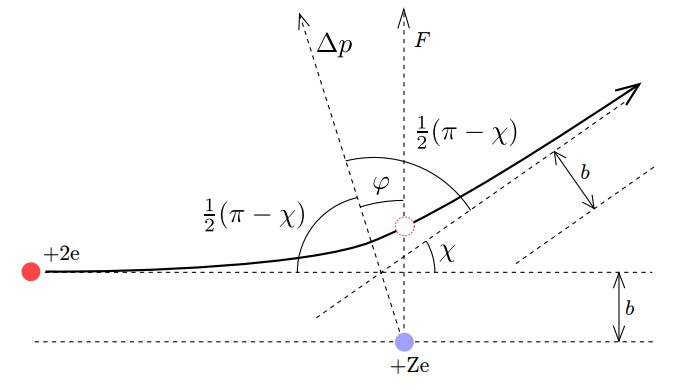
\includegraphics[width=0.49\textwidth]{rozptyl.jpg}
    \caption{Schéma rozptylu $ \alpha $-částice. }
\end{figure}

\section{Postup měření}

Uspořádání experimentu je znázorněné na obrázku 2. Ze zdroje $ \alpha $-částic vyletuje do všech směrů v pravidelném množství $ N_0 $ částic za jednotku času a ty které se trefí na proužek folie mají nějakou šanci se odrazit k detektoru. S uvážením vztahu (1) by se mělo jejich celkové množství za jednotku času řídit vztahem

\begin{equation}
n = K \frac{\cos \alpha \cos \beta}{r_1^2 r_2^2 \sin^{4} \frac{\chi}{2}},
\end{equation}

\noindent
kde $ K $ je konstanta daná experimentálním uspořádáním. Pro ověření tohoto vztahu nejdřív vyjádřím pravou stranu jako koeficient $ \omega $ v vynásobené konstantou $ K $ a změřím, jestli je tato závislost opravdu lineární.

\begin{equation}
n = K \omega
\end{equation}

\begin{figure}[htpb]
    \centering
    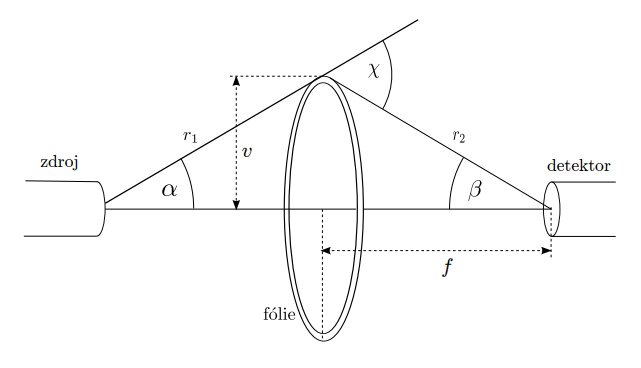
\includegraphics[width=0.7\textwidth]{aparatura.jpg}
    \caption{Experimentální uspořádání aparatury}
\end{figure}

\subsection{Poissonovo rozdělení}

Rozpad atomů je čistě náhodný proces, takže by se měl i řídit Poissonovým rozdělením  

\begin{equation}
P(n) = \frac{\lambda^{n}}{n!}e^{-\lambda},
\end{equation}

\noindent
kde $ P(n) $  je pravděpodobnost, že dojde k n rozpadům za časový interval a $ \lambda $  je střední hodnota počtu zaznamenaných rozpadů během měřícího intervalu. Ověření, že rozpady opravdu odpovídají tomuto rozdělení proběhne následovně. Dlouhé měření rozpadů rozdělím na $ N $  stejných časových úseků délky $ T $ a pro každý zjistím počet zaznamenaných částic $ n $ a střední hodnotu $ \lambda = \bar{n}  $. Četnost všech $ n $ označím jako $ K ( n ) $, pro které by mělo přibližně platit $ N P(n) \approx K(n) $.

Vyhodnocení dál proběhne metodou $ \chi $  kvadrátu. V případě, že pro nějaké $ n $  platí $ N P_{j} < 5 $ , pak tyto body sloučím s některým z okolních pro $ K_j(n) $ a $ P_j(n) $, tak aby byla splněná podmínka. Zbývá spočítat hodnotu $ \chi^2 $

\begin{equation}
\chi^2 = \sum_{j} \frac{\left( K_j(n) - N P_j(n) \right)^2 }{ N P_j(n)}.
\end{equation}

\noindent
a najít v tabulce hraniční $ \chi_{cr}^2 $ pro požadovanou hladinu spolehlivosti a stupně volnosti  $ n_{max}-1 $. Pokud je $ \chi^2 > \chi_{cr}^2 $, tak se rozpady Poissonovým rozdělením neřídí.
\newpage

\section{Výsledky měření}

Aparatura pro měření byla už připravená a jen jsem odečetl její rozměry. Vzdálenost mezi zdrojem a detektorem byla $ d = 22.7 $ cm a poloměr zlaté folie $ v = 2 $ cm. Pro několik poloh $ f $ jsem měřil čas, za který na detektor dopadlo 40 částic, a tyto hodnoty uvedl do tabulky 1. Ze vztahu (2) vyplývá, že počet dopadajících částic by měl být symetrický vzhledem ke střední poloze $ \frac{d}{2} = 11.7 $  cm, takže  jsem měřil jen jednu stranu.


\begin{table}[htpb]
    \centering
    \begin{tabular}{| c c c c c |}
        \hline
        $ f $  (cm) & $ t $ (s) &  počet částic & $ n $ (s$^{-1}  $ ) &  $ \omega \cdot 10^{6} $ (m$ ^{-4}  $ )  \\
        \hline
        11 &  91  & 40 & 0.440 & 6.05 \\
        12 &  102 & 40 & 0.392 & 6.02 \\
        13 &  95  & 40 & 0.421 & 5.80 \\
        14 &  107 & 40 & 0.374 & 5.41 \\
        15 &  147 & 40 & 0.272 & 4.86 \\
        16 &  140 & 40 & 0.286 & 4.17 \\
        17 &  90  & 15 & 0.167 & 3.40 \\
        18 &  403 & 43 & 0.141 & 2.58 \\
        19 &  408 & 38 & 0.093 & 1.77 \\
        20 &  455 & 40 & 0.088 & 1.04 \\
        \hline
    \end{tabular}
    \caption{Změřená data četnosti dopadajících $ \alpha $-částic }
    
\end{table}

Z naměřených hodnot jsem potom podle vztahu (2) vypočítal hodnoty $ \omega $ a vykreslil je do grafu 1. Fit byl přímkou, ze kterého jsem dostal hodnotu

\begin{equation}
K = (6.6 \pm 0.2) \cdot 10^{-8} \text{ m}^{4}\text{s}^{-1}
\end{equation}

\noindent
a s ní vykreslil teoretickou závislost $ n(f) $ do grafu 2 i s naměřenými hodnotami.  Grafy opravdu přibližně kopírují teoretické závislosti, ale měření nebylo dostatečně dlouhé, aby se dalo spolehlivě rozhodnout. Podle návodu k praktiku by mělo ve střední pozici na detektor dopadat 30 částic za sekundu, což vede spíš na hodnotu 

\begin{equation}
K = 8.248  \cdot 10^{-8} \text{ m}^{4}\text{s}^{-1}
\end{equation}

\noindent
a grafy by byly o kousek vyšší. V každém případě ale není možné změřená data vysvětlit Thompsonovým modelem. 

\begin{table}[htpb]
    \begin{minipage}[b]{.48\linewidth}
        \centering
        \resizebox{\textwidth}{!}{ % GNUPLOT: LaTeX picture with Postscript
\begingroup
  \makeatletter
  \providecommand\color[2][]{%
    \GenericError{(gnuplot) \space\space\space\@spaces}{%
      Package color not loaded in conjunction with
      terminal option `colourtext'%
    }{See the gnuplot documentation for explanation.%
    }{Either use 'blacktext' in gnuplot or load the package
      color.sty in LaTeX.}%
    \renewcommand\color[2][]{}%
  }%
  \providecommand\includegraphics[2][]{%
    \GenericError{(gnuplot) \space\space\space\@spaces}{%
      Package graphicx or graphics not loaded%
    }{See the gnuplot documentation for explanation.%
    }{The gnuplot epslatex terminal needs graphicx.sty or graphics.sty.}%
    \renewcommand\includegraphics[2][]{}%
  }%
  \providecommand\rotatebox[2]{#2}%
  \@ifundefined{ifGPcolor}{%
    \newif\ifGPcolor
    \GPcolorfalse
  }{}%
  \@ifundefined{ifGPblacktext}{%
    \newif\ifGPblacktext
    \GPblacktexttrue
  }{}%
  % define a \g@addto@macro without @ in the name:
  \let\gplgaddtomacro\g@addto@macro
  % define empty templates for all commands taking text:
  \gdef\gplbacktext{}%
  \gdef\gplfronttext{}%
  \makeatother
  \ifGPblacktext
    % no textcolor at all
    \def\colorrgb#1{}%
    \def\colorgray#1{}%
  \else
    % gray or color?
    \ifGPcolor
      \def\colorrgb#1{\color[rgb]{#1}}%
      \def\colorgray#1{\color[gray]{#1}}%
      \expandafter\def\csname LTw\endcsname{\color{white}}%
      \expandafter\def\csname LTb\endcsname{\color{black}}%
      \expandafter\def\csname LTa\endcsname{\color{black}}%
      \expandafter\def\csname LT0\endcsname{\color[rgb]{1,0,0}}%
      \expandafter\def\csname LT1\endcsname{\color[rgb]{0,1,0}}%
      \expandafter\def\csname LT2\endcsname{\color[rgb]{0,0,1}}%
      \expandafter\def\csname LT3\endcsname{\color[rgb]{1,0,1}}%
      \expandafter\def\csname LT4\endcsname{\color[rgb]{0,1,1}}%
      \expandafter\def\csname LT5\endcsname{\color[rgb]{1,1,0}}%
      \expandafter\def\csname LT6\endcsname{\color[rgb]{0,0,0}}%
      \expandafter\def\csname LT7\endcsname{\color[rgb]{1,0.3,0}}%
      \expandafter\def\csname LT8\endcsname{\color[rgb]{0.5,0.5,0.5}}%
    \else
      % gray
      \def\colorrgb#1{\color{black}}%
      \def\colorgray#1{\color[gray]{#1}}%
      \expandafter\def\csname LTw\endcsname{\color{white}}%
      \expandafter\def\csname LTb\endcsname{\color{black}}%
      \expandafter\def\csname LTa\endcsname{\color{black}}%
      \expandafter\def\csname LT0\endcsname{\color{black}}%
      \expandafter\def\csname LT1\endcsname{\color{black}}%
      \expandafter\def\csname LT2\endcsname{\color{black}}%
      \expandafter\def\csname LT3\endcsname{\color{black}}%
      \expandafter\def\csname LT4\endcsname{\color{black}}%
      \expandafter\def\csname LT5\endcsname{\color{black}}%
      \expandafter\def\csname LT6\endcsname{\color{black}}%
      \expandafter\def\csname LT7\endcsname{\color{black}}%
      \expandafter\def\csname LT8\endcsname{\color{black}}%
    \fi
  \fi
    \setlength{\unitlength}{0.0500bp}%
    \ifx\gptboxheight\undefined%
      \newlength{\gptboxheight}%
      \newlength{\gptboxwidth}%
      \newsavebox{\gptboxtext}%
    \fi%
    \setlength{\fboxrule}{0.5pt}%
    \setlength{\fboxsep}{1pt}%
    \definecolor{tbcol}{rgb}{1,1,1}%
\begin{picture}(5328.00,3600.00)%
    \gplgaddtomacro\gplbacktext{%
      \csname LTb\endcsname%%
      \put(814,704){\makebox(0,0)[r]{\strut{}$0$}}%
      \put(814,1239){\makebox(0,0)[r]{\strut{}$0.1$}}%
      \put(814,1774){\makebox(0,0)[r]{\strut{}$0.2$}}%
      \put(814,2309){\makebox(0,0)[r]{\strut{}$0.3$}}%
      \put(814,2844){\makebox(0,0)[r]{\strut{}$0.4$}}%
      \put(814,3379){\makebox(0,0)[r]{\strut{}$0.5$}}%
      \put(946,484){\makebox(0,0){\strut{}$1$}}%
      \put(1610,484){\makebox(0,0){\strut{}$2$}}%
      \put(2274,484){\makebox(0,0){\strut{}$3$}}%
      \put(2939,484){\makebox(0,0){\strut{}$4$}}%
      \put(3603,484){\makebox(0,0){\strut{}$5$}}%
      \put(4267,484){\makebox(0,0){\strut{}$6$}}%
      \put(4931,484){\makebox(0,0){\strut{}$7$}}%
    }%
    \gplgaddtomacro\gplfronttext{%
      \csname LTb\endcsname%%
      \put(209,2041){\rotatebox{-270}{\makebox(0,0){\strut{}$n$ (s$^{-1}$)}}}%
      \put(2938,154){\makebox(0,0){\strut{}$\omega \cdot 10^6$ (m$^{-4}$)}}%
      \csname LTb\endcsname%%
      \put(3944,3206){\makebox(0,0)[r]{\strut{}fit}}%
    }%
    \gplbacktext
    \put(0,0){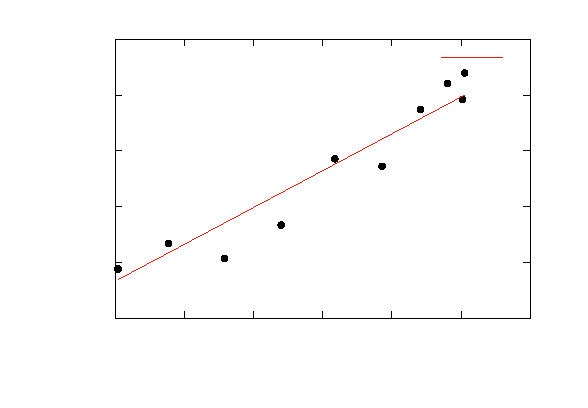
\includegraphics[width={266.40bp},height={180.00bp}]{cetnost}}%
    \gplfronttext
  \end{picture}%
\endgroup
 }
        \captionsetup{type=graph}
        \caption{ Závislost počtu dopadajících částic na $ \omega $  }
    \end{minipage} 
    \hfill
    \begin{minipage}[b]{.48\linewidth}
        \centering
        \resizebox{\textwidth}{!}{ % GNUPLOT: LaTeX picture with Postscript
\begingroup
  \makeatletter
  \providecommand\color[2][]{%
    \GenericError{(gnuplot) \space\space\space\@spaces}{%
      Package color not loaded in conjunction with
      terminal option `colourtext'%
    }{See the gnuplot documentation for explanation.%
    }{Either use 'blacktext' in gnuplot or load the package
      color.sty in LaTeX.}%
    \renewcommand\color[2][]{}%
  }%
  \providecommand\includegraphics[2][]{%
    \GenericError{(gnuplot) \space\space\space\@spaces}{%
      Package graphicx or graphics not loaded%
    }{See the gnuplot documentation for explanation.%
    }{The gnuplot epslatex terminal needs graphicx.sty or graphics.sty.}%
    \renewcommand\includegraphics[2][]{}%
  }%
  \providecommand\rotatebox[2]{#2}%
  \@ifundefined{ifGPcolor}{%
    \newif\ifGPcolor
    \GPcolorfalse
  }{}%
  \@ifundefined{ifGPblacktext}{%
    \newif\ifGPblacktext
    \GPblacktexttrue
  }{}%
  % define a \g@addto@macro without @ in the name:
  \let\gplgaddtomacro\g@addto@macro
  % define empty templates for all commands taking text:
  \gdef\gplbacktext{}%
  \gdef\gplfronttext{}%
  \makeatother
  \ifGPblacktext
    % no textcolor at all
    \def\colorrgb#1{}%
    \def\colorgray#1{}%
  \else
    % gray or color?
    \ifGPcolor
      \def\colorrgb#1{\color[rgb]{#1}}%
      \def\colorgray#1{\color[gray]{#1}}%
      \expandafter\def\csname LTw\endcsname{\color{white}}%
      \expandafter\def\csname LTb\endcsname{\color{black}}%
      \expandafter\def\csname LTa\endcsname{\color{black}}%
      \expandafter\def\csname LT0\endcsname{\color[rgb]{1,0,0}}%
      \expandafter\def\csname LT1\endcsname{\color[rgb]{0,1,0}}%
      \expandafter\def\csname LT2\endcsname{\color[rgb]{0,0,1}}%
      \expandafter\def\csname LT3\endcsname{\color[rgb]{1,0,1}}%
      \expandafter\def\csname LT4\endcsname{\color[rgb]{0,1,1}}%
      \expandafter\def\csname LT5\endcsname{\color[rgb]{1,1,0}}%
      \expandafter\def\csname LT6\endcsname{\color[rgb]{0,0,0}}%
      \expandafter\def\csname LT7\endcsname{\color[rgb]{1,0.3,0}}%
      \expandafter\def\csname LT8\endcsname{\color[rgb]{0.5,0.5,0.5}}%
    \else
      % gray
      \def\colorrgb#1{\color{black}}%
      \def\colorgray#1{\color[gray]{#1}}%
      \expandafter\def\csname LTw\endcsname{\color{white}}%
      \expandafter\def\csname LTb\endcsname{\color{black}}%
      \expandafter\def\csname LTa\endcsname{\color{black}}%
      \expandafter\def\csname LT0\endcsname{\color{black}}%
      \expandafter\def\csname LT1\endcsname{\color{black}}%
      \expandafter\def\csname LT2\endcsname{\color{black}}%
      \expandafter\def\csname LT3\endcsname{\color{black}}%
      \expandafter\def\csname LT4\endcsname{\color{black}}%
      \expandafter\def\csname LT5\endcsname{\color{black}}%
      \expandafter\def\csname LT6\endcsname{\color{black}}%
      \expandafter\def\csname LT7\endcsname{\color{black}}%
      \expandafter\def\csname LT8\endcsname{\color{black}}%
    \fi
  \fi
    \setlength{\unitlength}{0.0500bp}%
    \ifx\gptboxheight\undefined%
      \newlength{\gptboxheight}%
      \newlength{\gptboxwidth}%
      \newsavebox{\gptboxtext}%
    \fi%
    \setlength{\fboxrule}{0.5pt}%
    \setlength{\fboxsep}{1pt}%
    \definecolor{tbcol}{rgb}{1,1,1}%
\begin{picture}(5328.00,3600.00)%
    \gplgaddtomacro\gplbacktext{%
      \csname LTb\endcsname%%
      \put(462,440){\makebox(0,0)[r]{\strut{}$0$}}%
      \put(462,930){\makebox(0,0)[r]{\strut{}$5$}}%
      \put(462,1420){\makebox(0,0)[r]{\strut{}$10$}}%
      \put(462,1910){\makebox(0,0)[r]{\strut{}$15$}}%
      \put(462,2399){\makebox(0,0)[r]{\strut{}$20$}}%
      \put(462,2889){\makebox(0,0)[r]{\strut{}$25$}}%
      \put(462,3379){\makebox(0,0)[r]{\strut{}$30$}}%
      \put(594,220){\makebox(0,0){\strut{}$11$}}%
      \put(1076,220){\makebox(0,0){\strut{}$12$}}%
      \put(1558,220){\makebox(0,0){\strut{}$13$}}%
      \put(2040,220){\makebox(0,0){\strut{}$14$}}%
      \put(2522,220){\makebox(0,0){\strut{}$15$}}%
      \put(3003,220){\makebox(0,0){\strut{}$16$}}%
      \put(3485,220){\makebox(0,0){\strut{}$17$}}%
      \put(3967,220){\makebox(0,0){\strut{}$18$}}%
      \put(4449,220){\makebox(0,0){\strut{}$19$}}%
      \put(4931,220){\makebox(0,0){\strut{}$20$}}%
    }%
    \gplgaddtomacro\gplfronttext{%
      \csname LTb\endcsname%%
      \put(99,1909){\rotatebox{-270}{\makebox(0,0){\strut{}}}}%
      \put(2762,-66){\makebox(0,0){\strut{}}}%
    }%
    \gplbacktext
    \put(0,0){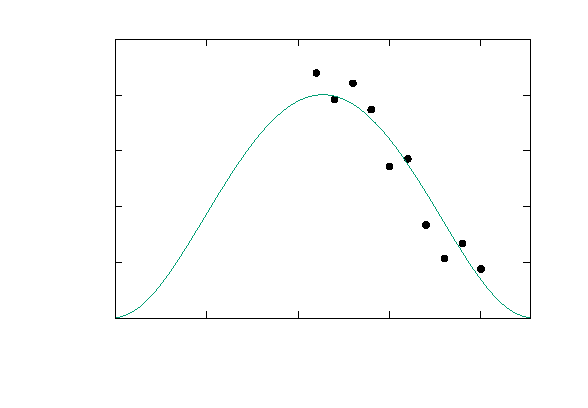
\includegraphics[width={266.40bp},height={180.00bp}]{data}}%
    \gplfronttext
  \end{picture}%
\endgroup
 }
        \captionsetup{type=graph}
        \caption{ Závislost počtu dopadajících částic na $ f $  }
    \end{minipage} 
\end{table}

\subsection{Poissonovo rozdělení rozpadu $ \alpha $ částic }

Folii jsem přesunul doprostřed, aby se zaznamenávalo co nejvíce rozpadů, a po dobu 850 s zapisoval časy detekovaných částic. Podle postupu výpočtu $ \chi $ kvadrátu jsem potom sestavil tabulku 2 a vykreslil teoretické Poissonovo rozdělení vůči vypočítanému do grafu 3. Před vyhodnocením musím sloučit řádky pro $ n = 0-2 $ a  $ n = 8-12 $, aby platili podmínky $ \chi^2 $ testu, odkud potom podle vztahu (5) vychází

\begin{equation}
\chi^2 = 5.97
\end{equation}

Hodnota $ \chi_{cr} $ pro hladinu spolehlivost $ 0.05 $ a $ 12 - 1 = 11 $ stupňů volnosti je $ \chi_{cr} = 19.675 $, což je větší než $ \chi^2 $, takže test vychází pozitivně. 

\begin{table}[htpb]
    \begin{minipage}[b]{.48\linewidth}
        \centering
        \begin{tabular}{|  r @{\hspace{20pt}} c @{\hspace{20pt}} r @{\hspace{20pt}} c | }
            \hline
            $ n $  & $ K(n) $ & $ P(n) $ & $ K(n) \approx P(n) \cdot N $ \\ 
            \hline
            0  & 2  & 0.013 & 1.7  \\
            1  & 7  & 0.056 & 7.3  \\
            2  & 20 & 0.122 & 15.9 \\
            3  & 22 & 0.177 & 23.0 \\
            4  & 25 & 0.193 & 25.0 \\
            5  & 25 & 0.167 & 21.8 \\
            6  & 15 & 0.121 & 15.8 \\
            7  & 3  & 0.075 & 9.79 \\
            8  & 6  & 0.041 & 5.32 \\
            10 & 1  & 0.020 & 2.57 \\
            11 & 2  & 0.009 & 1.12 \\
            12 & 1  & 0.003 & 0.44 \\
            \hline
        \end{tabular}
        \caption{Vyhodnocování testu $ \chi^2 $ pro $ N = 130  $ a $ \lambda = 0.43 $ částic $ s^{-1} $.  }
    \end{minipage} 
    \hfill
    \begin{minipage}[b]{.50\linewidth}
        \centering
        \resizebox{\textwidth}{!}{ % GNUPLOT: LaTeX picture with Postscript
\begingroup
  \makeatletter
  \providecommand\color[2][]{%
    \GenericError{(gnuplot) \space\space\space\@spaces}{%
      Package color not loaded in conjunction with
      terminal option `colourtext'%
    }{See the gnuplot documentation for explanation.%
    }{Either use 'blacktext' in gnuplot or load the package
      color.sty in LaTeX.}%
    \renewcommand\color[2][]{}%
  }%
  \providecommand\includegraphics[2][]{%
    \GenericError{(gnuplot) \space\space\space\@spaces}{%
      Package graphicx or graphics not loaded%
    }{See the gnuplot documentation for explanation.%
    }{The gnuplot epslatex terminal needs graphicx.sty or graphics.sty.}%
    \renewcommand\includegraphics[2][]{}%
  }%
  \providecommand\rotatebox[2]{#2}%
  \@ifundefined{ifGPcolor}{%
    \newif\ifGPcolor
    \GPcolorfalse
  }{}%
  \@ifundefined{ifGPblacktext}{%
    \newif\ifGPblacktext
    \GPblacktexttrue
  }{}%
  % define a \g@addto@macro without @ in the name:
  \let\gplgaddtomacro\g@addto@macro
  % define empty templates for all commands taking text:
  \gdef\gplbacktext{}%
  \gdef\gplfronttext{}%
  \makeatother
  \ifGPblacktext
    % no textcolor at all
    \def\colorrgb#1{}%
    \def\colorgray#1{}%
  \else
    % gray or color?
    \ifGPcolor
      \def\colorrgb#1{\color[rgb]{#1}}%
      \def\colorgray#1{\color[gray]{#1}}%
      \expandafter\def\csname LTw\endcsname{\color{white}}%
      \expandafter\def\csname LTb\endcsname{\color{black}}%
      \expandafter\def\csname LTa\endcsname{\color{black}}%
      \expandafter\def\csname LT0\endcsname{\color[rgb]{1,0,0}}%
      \expandafter\def\csname LT1\endcsname{\color[rgb]{0,1,0}}%
      \expandafter\def\csname LT2\endcsname{\color[rgb]{0,0,1}}%
      \expandafter\def\csname LT3\endcsname{\color[rgb]{1,0,1}}%
      \expandafter\def\csname LT4\endcsname{\color[rgb]{0,1,1}}%
      \expandafter\def\csname LT5\endcsname{\color[rgb]{1,1,0}}%
      \expandafter\def\csname LT6\endcsname{\color[rgb]{0,0,0}}%
      \expandafter\def\csname LT7\endcsname{\color[rgb]{1,0.3,0}}%
      \expandafter\def\csname LT8\endcsname{\color[rgb]{0.5,0.5,0.5}}%
    \else
      % gray
      \def\colorrgb#1{\color{black}}%
      \def\colorgray#1{\color[gray]{#1}}%
      \expandafter\def\csname LTw\endcsname{\color{white}}%
      \expandafter\def\csname LTb\endcsname{\color{black}}%
      \expandafter\def\csname LTa\endcsname{\color{black}}%
      \expandafter\def\csname LT0\endcsname{\color{black}}%
      \expandafter\def\csname LT1\endcsname{\color{black}}%
      \expandafter\def\csname LT2\endcsname{\color{black}}%
      \expandafter\def\csname LT3\endcsname{\color{black}}%
      \expandafter\def\csname LT4\endcsname{\color{black}}%
      \expandafter\def\csname LT5\endcsname{\color{black}}%
      \expandafter\def\csname LT6\endcsname{\color{black}}%
      \expandafter\def\csname LT7\endcsname{\color{black}}%
      \expandafter\def\csname LT8\endcsname{\color{black}}%
    \fi
  \fi
    \setlength{\unitlength}{0.0500bp}%
    \ifx\gptboxheight\undefined%
      \newlength{\gptboxheight}%
      \newlength{\gptboxwidth}%
      \newsavebox{\gptboxtext}%
    \fi%
    \setlength{\fboxrule}{0.5pt}%
    \setlength{\fboxsep}{1pt}%
    \definecolor{tbcol}{rgb}{1,1,1}%
\begin{picture}(5328.00,3600.00)%
    \gplgaddtomacro\gplbacktext{%
      \csname LTb\endcsname%%
      \put(682,704){\makebox(0,0)[r]{\strut{}$0$}}%
      \put(682,1150){\makebox(0,0)[r]{\strut{}$5$}}%
      \put(682,1596){\makebox(0,0)[r]{\strut{}$10$}}%
      \put(682,2042){\makebox(0,0)[r]{\strut{}$15$}}%
      \put(682,2487){\makebox(0,0)[r]{\strut{}$20$}}%
      \put(682,2933){\makebox(0,0)[r]{\strut{}$25$}}%
      \put(682,3379){\makebox(0,0)[r]{\strut{}$30$}}%
      \put(814,484){\makebox(0,0){\strut{}$0$}}%
      \put(1500,484){\makebox(0,0){\strut{}$2$}}%
      \put(2186,484){\makebox(0,0){\strut{}$4$}}%
      \put(2873,484){\makebox(0,0){\strut{}$6$}}%
      \put(3559,484){\makebox(0,0){\strut{}$8$}}%
      \put(4245,484){\makebox(0,0){\strut{}$10$}}%
      \put(4931,484){\makebox(0,0){\strut{}$12$}}%
    }%
    \gplgaddtomacro\gplfronttext{%
      \csname LTb\endcsname%%
      \put(209,2041){\rotatebox{-270}{\makebox(0,0){\strut{}$ K(n) $}}}%
      \put(2872,154){\makebox(0,0){\strut{}n}}%
      \csname LTb\endcsname%%
      \put(4406,3028){\makebox(0,0)[r]{\strut{}$ P(n) \cdot N  $ }}%
    }%
    \gplbacktext
    \put(0,0){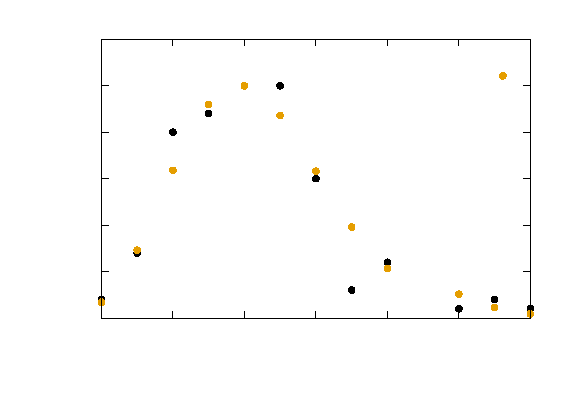
\includegraphics[width={266.40bp},height={180.00bp}]{poisson}}%
    \gplfronttext
  \end{picture}%
\endgroup
 }
        \captionsetup{type=graph}
        \caption{Poissonovo rozdělení rozpadu $ \alpha $-částic. }
        \vspace{20pt}
    \end{minipage} 
\end{table}

\section{Závěr}

Na aparatuře Rutherfordova experimentu jsem měřil množství částic odražených na velmi tenké zlaté folii o úhly $ \chi $, a zjistil, že změřená data se dají vysvětlit Rutherfordovým modelem atomu, zatímco ten Thompsonův toto nedokáže. 

Druhým úkolem bylo ověřit, že rozpad atomů na $ \alpha $-částice probíhá podle Poissonova rozdělení. K tomuto účelu jsem použil $ \chi^2 $ test, který vyšel pozitivně pro hladinu spolehlivosti alespoň $ 0.05 $. Pro lepší spolehlivost by bylo potřeba měřit mnohem déle. Na to ale v praktiku už nezbyl čas. 

\begin{thebibliography}{0}
\bibitem{tabulky} Hustota pevných látek. Dostupné z~\url{http://www.converter.cz/tabulky/hustota-pevne.htmf}.   
\end{thebibliography}

\end{document}
